\chapter{Anexos}

El presente capítulo agrupa la documentación complementaria que respalda
la operación, mantenimiento y trazabilidad de la red instalada.

\section{Manual de operación y mantenimiento}

El manual de operación y mantenimiento constituye la guía de referencia
para la administración de la red a lo largo de su vida útil. Contempla
los siguientes contenidos:

\begin{itemize}
\item \textbf{Descripción de la red:} topología en estrella jerárquica,
ubicación del MDF y los IDF, y esquema de distribución por niveles.
\item \textbf{Procedimientos de operación:} encendido y apagado
ordenado de equipos activos, gestión de los UPS y verificación de
estados de conexión.
\item \textbf{Mantenimiento preventivo:} inspección periódica de
gabinetes, limpieza de filtros de ventilación, revisión del sistema de
puesta a tierra (resistencia $\leq$5\,\textohm) y verificación del
etiquetado.
\item \textbf{Mantenimiento correctivo:} protocolo de diagnóstico ante
fallas de enlace, uso del certificador y re-terminación de puntos
defectuosos.
\item \textbf{Registro de administración:} actualización de la base de
datos de puntos bajo la norma ANSI/TIA-606-C ante cualquier
modificación.
\end{itemize}

\section{Diagramas de red lógica y física}

Se incluyen los diagramas que representan la arquitectura de la red
tanto en su dimensión física (rutas, gabinetes y puntos) como lógica
(segmentación y flujo de datos entre el MDF y los IDF).

% =============================================================
% >>> IMAGEN: DIAGRAMA DE RED FÍSICA Y LÓGICA <<<
% Insertar aquí el/los diagrama(s) de red. Sugerencia:
% \begin{figure}[H]
%   \centering
%   \includegraphics[width=\textwidth]{DiagramaRedLogica.png}
%   \caption{Diagrama lógico de la red del pabellón de Informática.}
% \end{figure}
% =============================================================

\subsection{Fichas técnicas de equipos y materiales}

A continuación se presentan las fichas técnicas de los principales equipos y
materiales especificados en el proyecto, con su respectiva referencia visual. Las
imágenes se encuentran en la carpeta \texttt{Componentes/} del repositorio del
proyecto; solo debe ajustarse el nombre de archivo en cada
\texttt{\textbackslash includegraphics}.

% ------------------------------------------------------------------
% Plantilla reutilizable: descripción a la izquierda, imagen a la derecha.
% Copiar este bloque por cada equipo y cambiar los campos marcados.
% ------------------------------------------------------------------

\subsubsection*{Cableado y conectividad}

\begin{table}[H]
\centering
\renewcommand{\arraystretch}{1.3}
\begin{tabular}{p{9cm} p{4.5cm}}
\textbf{Cable F/UTP Cat 6A LSZH} \newline
\textit{Marca: Panduit --- Modelo: PUFL6X04WH --- Caja 305m} \newline
Cable de cobre para cableado horizontal, foliado (F/UTP), cubierta LSZH libre de halógenos. Certificación de canal Categoría 6A hasta 500 MHz. &
\centering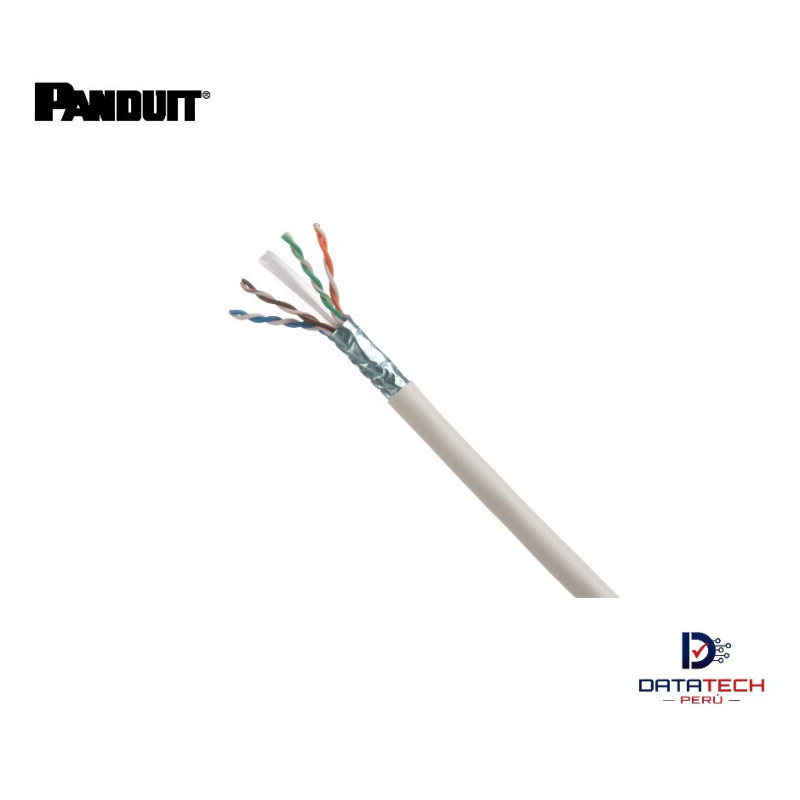
\includegraphics[width=4cm]{Componentes/01_cable_cat6a.jpg} \\
\end{tabular}
\end{table}

\begin{table}[H]
\centering
\renewcommand{\arraystretch}{1.3}
\begin{tabular}{p{9cm} p{4.5cm}}
\textbf{Patch Panel Modular 24P} \newline
\textit{Marca: CommScope --- Modelo: 760237040} \newline
Panel de conexión de 24 puertos, vacío/modular, para instalación en gabinetes MDF e IDF. &
\centering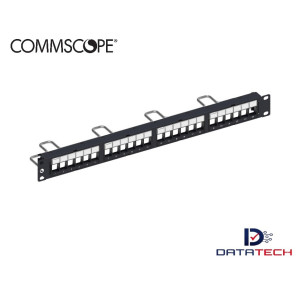
\includegraphics[width=4cm]{Componentes/02_patchpanel_24p.jpg} \\
\end{tabular}
\end{table}

\begin{table}[H]
\centering
\renewcommand{\arraystretch}{1.3}
\begin{tabular}{p{9cm} p{4.5cm}}
\textbf{Jack RJ45 Cat 6A Blindado MiniCom} \newline
\textit{Marca: Panduit --- Modelo: CJS6X88TGY} \newline
Módulo de conexión blindado, terminación por desplazamiento de aislante (IDC), contacto de 50 micras de oro. &
\centering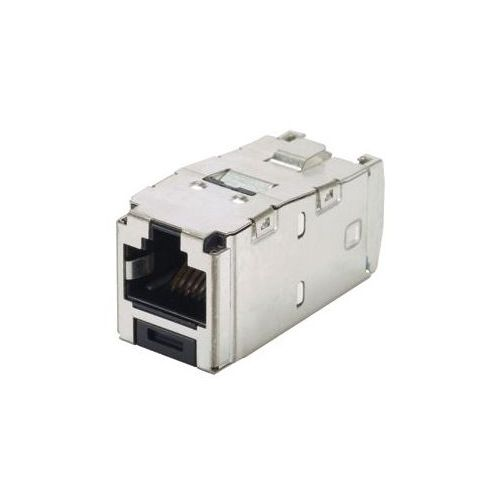
\includegraphics[width=4cm]{Componentes/03_jack_cat6a.jpg} \\
\end{tabular}
\end{table}

\begin{table}[H]
\centering
\renewcommand{\arraystretch}{1.3}
\begin{tabular}{p{9cm} p{4.5cm}}
\textbf{Patch Cord F/UTP Cat 6A 2.1m} \newline
\textit{Marca: Panduit --- Modelo: CO6X7BU} \newline
Cable de parcheo blindado, conectores RJ-45 moldeados con alivio de tensión. Uso: lado de usuario. &
\centering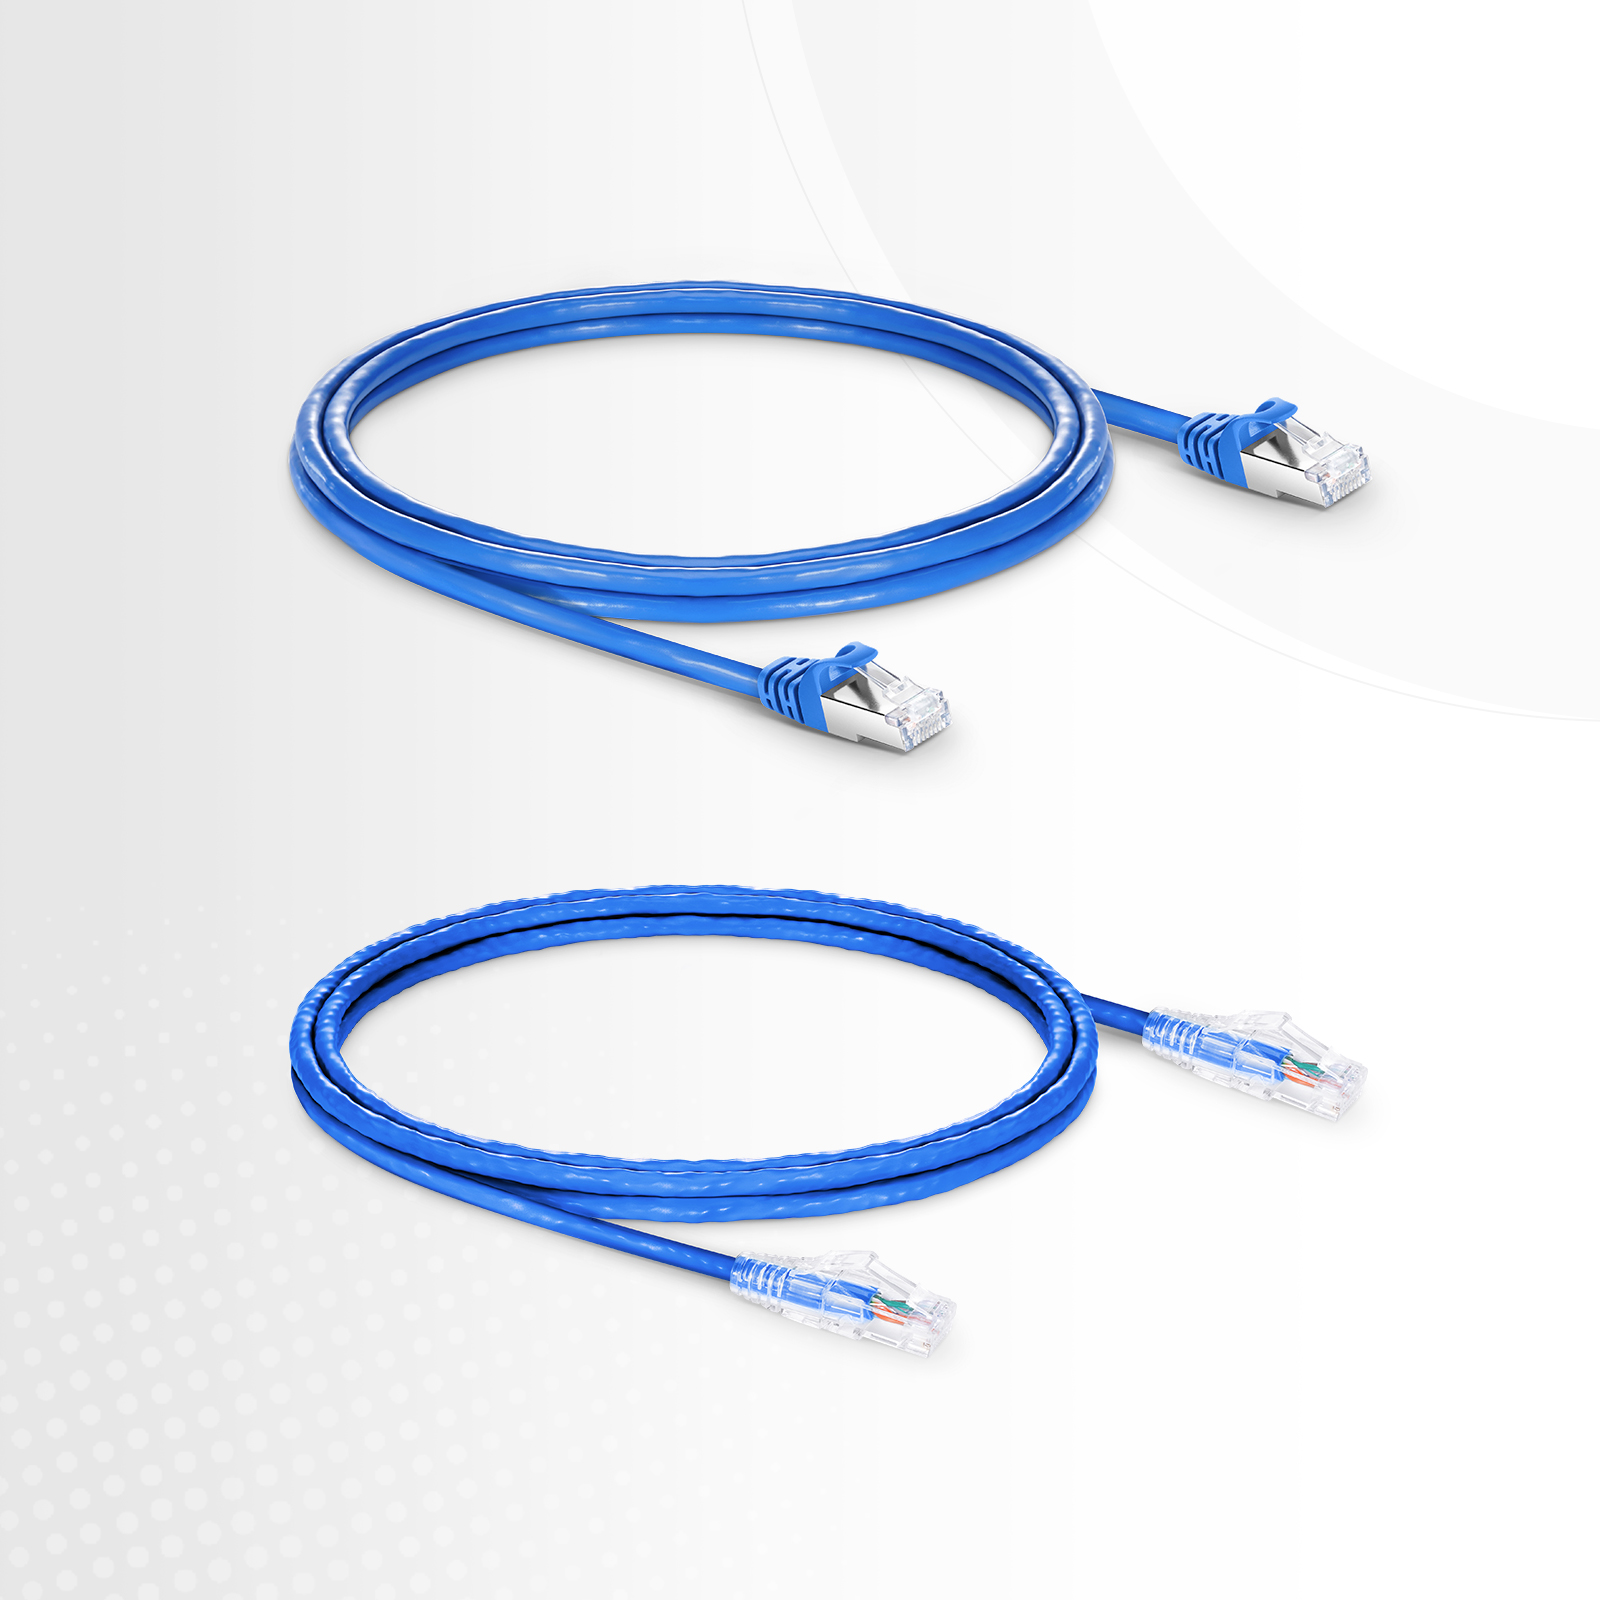
\includegraphics[width=4cm]{Componentes/04_patchcord_cat6a_2.1m.jpg} \\
\end{tabular}
\end{table}

\begin{table}[H]
\centering
\renewcommand{\arraystretch}{1.3}
\begin{tabular}{p{9cm} p{4.5cm}}
\textbf{Patch Cord F/UTP Cat 6A 1.0m} \newline
\textit{Marca: Panduit --- Modelo: CO6X3BU} \newline
Cable de parcheo blindado, conectores RJ-45 moldeados. Uso: lado de patch panel en gabinete. &
\centering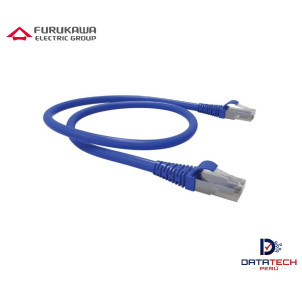
\includegraphics[width=4cm]{Componentes/05_patchcord_cat6a_1.0m.jpg} \\
\end{tabular}
\end{table}

\begin{table}[H]
\centering
\renewcommand{\arraystretch}{1.3}
\begin{tabular}{p{9cm} p{4.5cm}}
\textbf{Kit Fibra Óptica OM4} \newline
\textit{Marca: CommScope --- Serie: TeraSPEED} \newline
Fibra óptica multimodo de 4 hilos, chaqueta LSZH, optimizada para transmisión láser 10/40/100 Gbps. Backbone MDF--IDF. &
\centering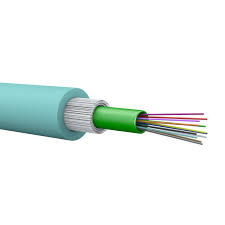
\includegraphics[width=4cm]{Componentes/06_kitfibraoptica_4hilos.jpg} \\
\end{tabular}
\end{table}

\begin{table}[H]
\centering
\renewcommand{\arraystretch}{1.3}
\begin{tabular}{p{9cm} p{4.5cm}}
\textbf{Faceplate 2 puertos} \newline
\textit{Marca: Panduit --- Modelo: CFPL2EIWH} \newline
Placa frontal color blanco con iconografía integrada para diferenciar datos, voz y CCTV. &
\centering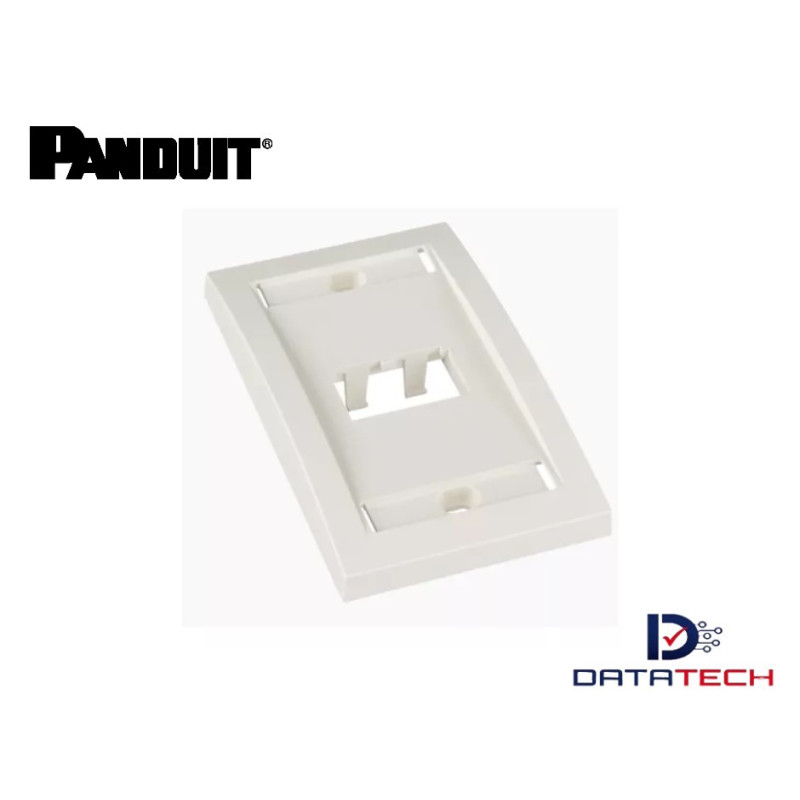
\includegraphics[width=4cm]{Componentes/07_faceplate_2puertos.jpg} \\
\end{tabular}
\end{table}

\begin{table}[H]
\centering
\renewcommand{\arraystretch}{1.3}
\begin{tabular}{p{9cm} p{4.5cm}}
\textbf{Caja Superficial PVC 1 Módulo} \newline
\textit{Marca: Panduit --- Modelo: CBX2EIWH} \newline
Caja de montaje superficial para faceplate, instalación sobre pared o canaleta. &
\centering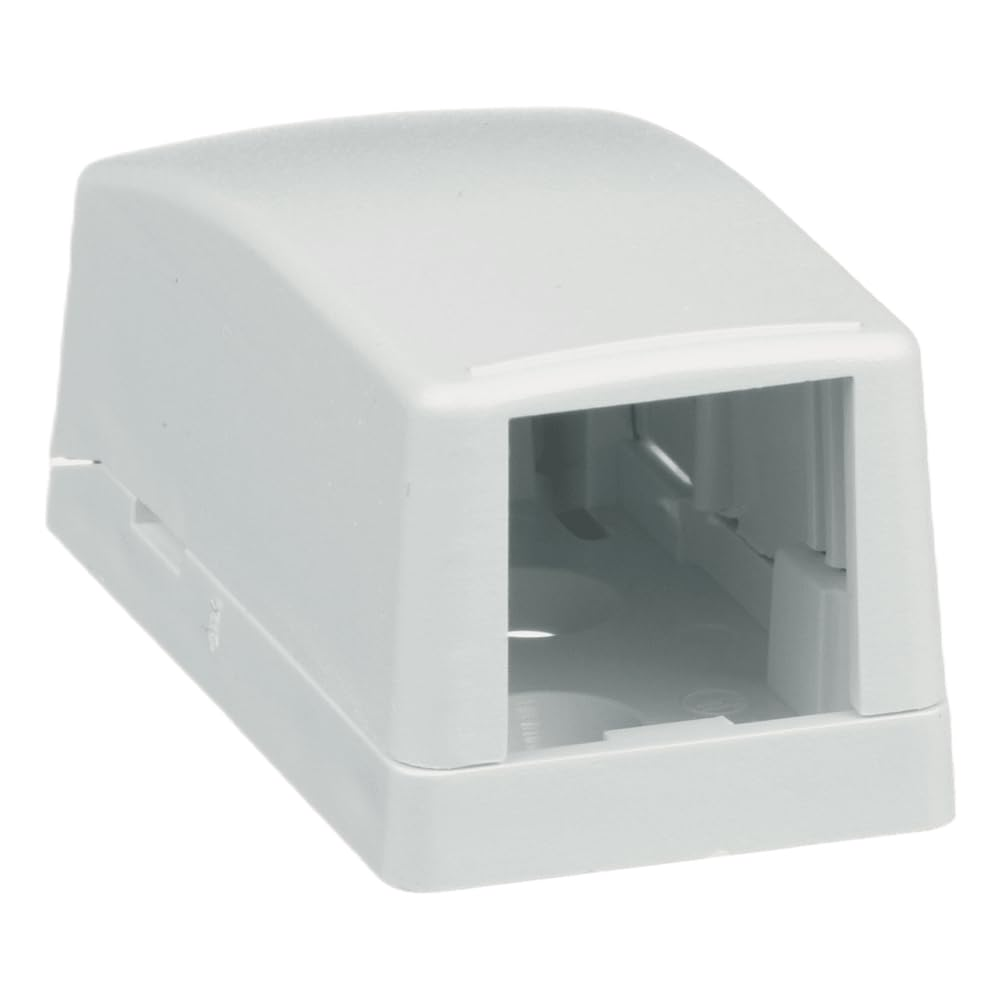
\includegraphics[width=4cm]{Componentes/08_cajasuperficial_1modulo.jpg} \\
\end{tabular}
\end{table}

\begin{table}[H]
\centering
\renewcommand{\arraystretch}{1.3}
\begin{tabular}{p{9cm} p{4.5cm}}
\textbf{Organizador Horizontal 1U} \newline
\textit{Marca: Tripp Lite --- Modelo: NR2600} \newline
Ducto ranurado frontal con tapa desmontable, instalado entre cada patch panel para guiado de cables. &
\centering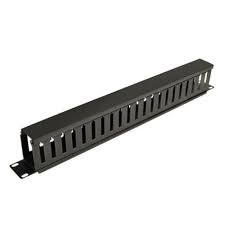
\includegraphics[width=4cm]{Componentes/09_organizadorhorizontal_1u.jpg} \\
\end{tabular}
\end{table}

\begin{table}[H]
\centering
\renewcommand{\arraystretch}{1.3}
\begin{tabular}{p{9cm} p{4.5cm}}
\textbf{Bandeja Porta-equipos 1U} \newline
\textit{Marca: Tripp Lite --- Modelo: RSD-1U} \newline
Bandeja estática para soporte de equipos no rackeables dentro del gabinete. &
\centering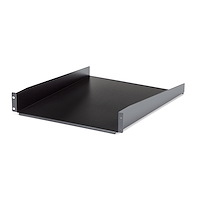
\includegraphics[width=4cm]{Componentes/10_bandejaportaequipos_1u.jpg} \\
\end{tabular}
\end{table}

\subsubsection*{Gabinetes de telecomunicaciones}

\begin{table}[H]
\centering
\renewcommand{\arraystretch}{1.3}
\begin{tabular}{p{9cm} p{4.5cm}}
\textbf{Gabinete de Piso 42U (MDF)} \newline
\textit{Marca: Tripp Lite --- Modelo: SR42UB} \newline
Gabinete cerrado de 19'' x 42U, puertas microperforadas, cerradura de seguridad. Ubicación: MDF-02, 2do piso. &
\centering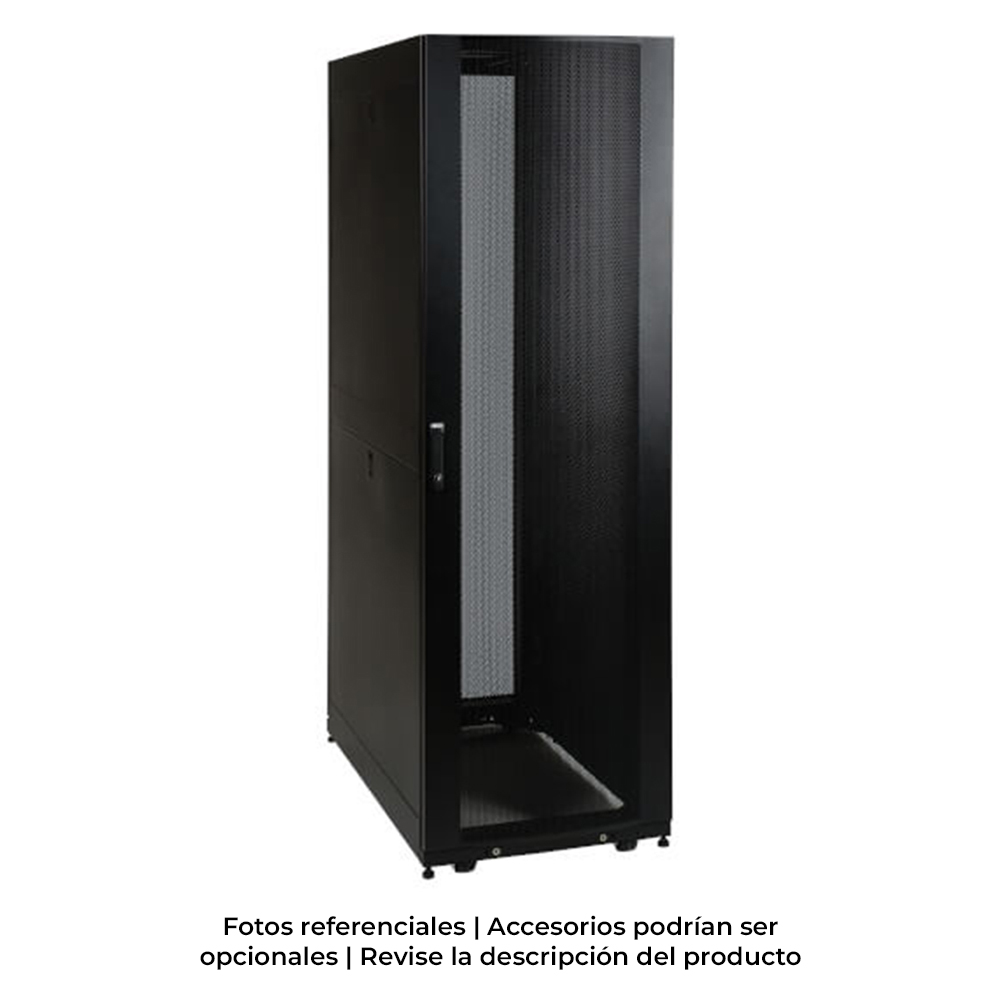
\includegraphics[width=4cm]{Componentes/11_gabinetepiso_42U.jpg} \\
\end{tabular}
\end{table}

\begin{table}[H]
\centering
\renewcommand{\arraystretch}{1.3}
\begin{tabular}{p{9cm} p{4.5cm}}
\textbf{Gabinete de Pared/Piso 24U (IDF)} \newline
\textit{Marca: Tripp Lite --- Modelo: SRW24US} \newline
Gabinete de 19'' x 24U. Se reutiliza este mismo modelo en los tres distribuidores de piso: IDF-01 (1er piso, nuevo), IDF-03 (3er piso) e IDF-04 (4to piso). &
\centering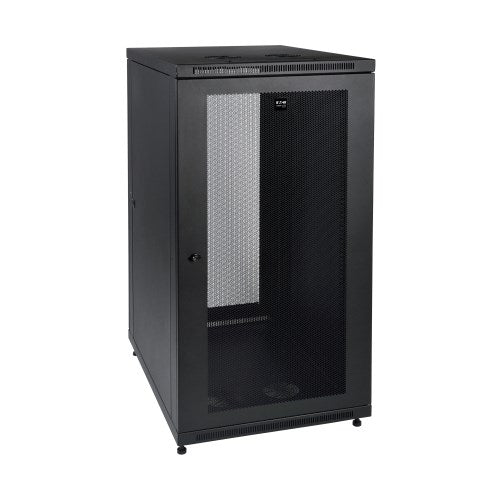
\includegraphics[width=4cm]{Componentes/12_gabinetepared_42U.jpg} \\
\end{tabular}
\end{table}

\subsubsection*{Puesta a tierra}

\begin{table}[H]
\centering
\renewcommand{\arraystretch}{1.3}
\begin{tabular}{p{9cm} p{4.5cm}}
\textbf{Barra de Tierra Principal (TMGB)} \newline
\textit{Marca: Panduit --- Modelo: TMGB-060} \newline
Barra de cobre perforada, punto de referencia de tierra para todo el sistema de telecomunicaciones. Ubicación: MDF, 2do piso. &
\centering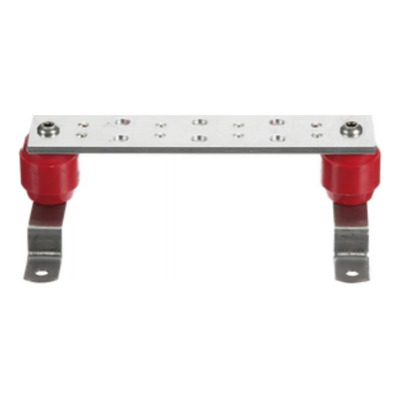
\includegraphics[width=4cm]{Componentes/13_barra_TMGB.jpg} \\
\end{tabular}
\end{table}

\begin{table}[H]
\centering
\renewcommand{\arraystretch}{1.3}
\begin{tabular}{p{9cm} p{4.5cm}}
\textbf{Barra de Tierra Secundaria (TGB)} \newline
\textit{Marca: Panduit --- Modelo: TGB-040} \newline
Barra secundaria instalada en cada IDF, interconectada a la TMGB. Se instalan 3 unidades (IDF-01, IDF-03, IDF-04). &
\centering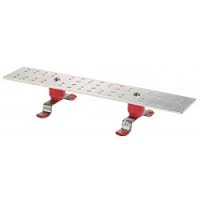
\includegraphics[width=4cm]{Componentes/14_barra_TGB.jpg} \\
\end{tabular}
\end{table}

\subsubsection*{Equipos activos}

\begin{table}[H]
\centering
\renewcommand{\arraystretch}{1.3}
\begin{tabular}{p{9cm} p{4.5cm}}
\textbf{Switch Catalyst 9200 48P PoE+} \newline
\textit{Marca: Cisco --- Modelo: C9200-48P-E} \newline
Switch de acceso Capa 2/3, 48 puertos PoE+, uplinks 10G SFP+ para backbone de fibra. &
\centering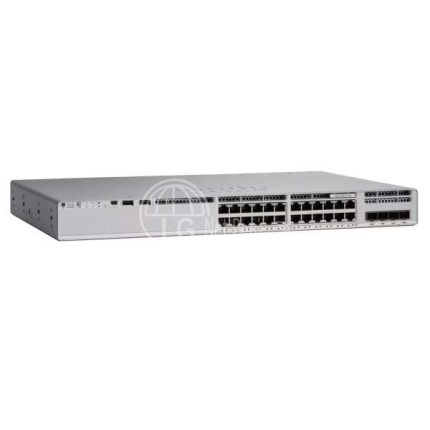
\includegraphics[width=4cm]{Componentes/15_switchcatalyst_ciscoc9200_24p.jpg} \\
\end{tabular}
\end{table}

\begin{table}[H]
\centering
\renewcommand{\arraystretch}{1.3}
\begin{tabular}{p{9cm} p{4.5cm}}
\textbf{Switch Catalyst 9200 24P PoE+} \newline
\textit{Marca: Cisco --- Modelo: C9200-24P-E} \newline
Switch de acceso 24 puertos PoE+, uplink 10G SFP+. Instalado en IDF-01 (1er piso, nuevo). &
\centering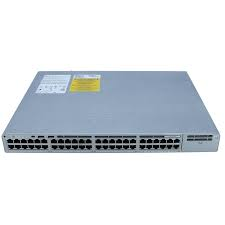
\includegraphics[width=4cm]{Componentes/16_switchcatalyst_ciscoc9200_48p.jpg} \\
\end{tabular}
\end{table}

\begin{table}[H]
\centering
\renewcommand{\arraystretch}{1.3}
\begin{tabular}{p{9cm} p{4.5cm}}
\textbf{Transceptor SFP+ 10G SR} \newline
\textit{Marca: Cisco --- Modelo: SFP-10G-SR} \newline
Módulo óptico multimodo para enlaces de backbone entre MDF y cada IDF. &
\centering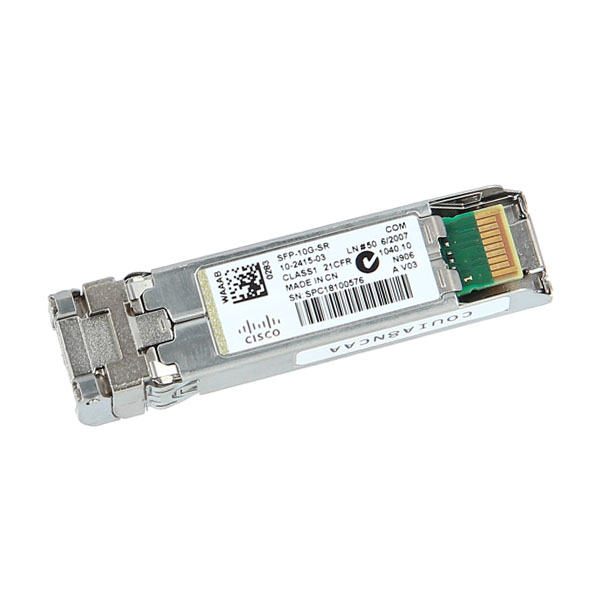
\includegraphics[width=4cm]{Componentes/17_transceptor_10gsr.jpg} \\
\end{tabular}
\end{table}

\begin{table}[H]
\centering
\renewcommand{\arraystretch}{1.3}
\begin{tabular}{p{9cm} p{4.5cm}}
\textbf{UPS Online 3kVA Rackeable} \newline
\textit{Marca: Tripp Lite --- Modelo: SU3000RTX} \newline
Sistema de alimentación ininterrumpida de doble conversión, autonomía mínima 15 min a plena carga. Uno por gabinete (4 unidades). &
\centering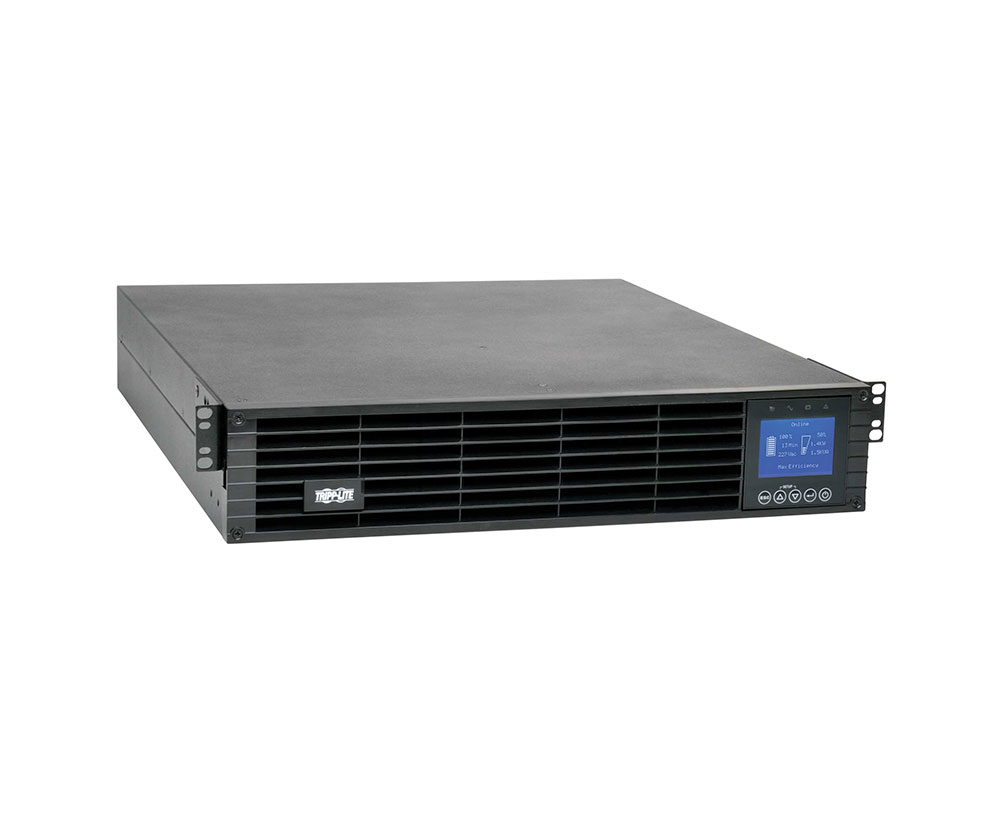
\includegraphics[width=4cm]{Componentes/18_upsonline_3kva.jpg} \\
\end{tabular}
\end{table}

\begin{table}[H]
\centering
\renewcommand{\arraystretch}{1.3}
\begin{tabular}{p{9cm} p{4.5cm}}
\textbf{Access Point WiFi 6 Interior} \newline
\textit{Marca: Cisco --- Modelo: C9120AXI} \newline
Punto de acceso doble banda, 802.11ax, alimentado por PoE+. &
\centering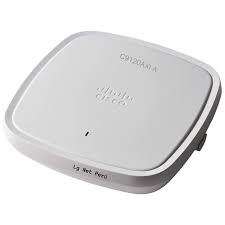
\includegraphics[width=4cm]{Componentes/19_accesspoint_wifi6.jpg} \\
\end{tabular}
\end{table}

\begin{table}[H]
\centering
\renewcommand{\arraystretch}{1.3}
\begin{tabular}{p{9cm} p{4.5cm}}
\textbf{Cámara IP Fija Interior 2MP} \newline
\textit{Marca: Dahua / Hikvision} \newline
Cámara IP con PoE+, resolución mínima 1920x1080, conectada a switches de acceso. &
\centering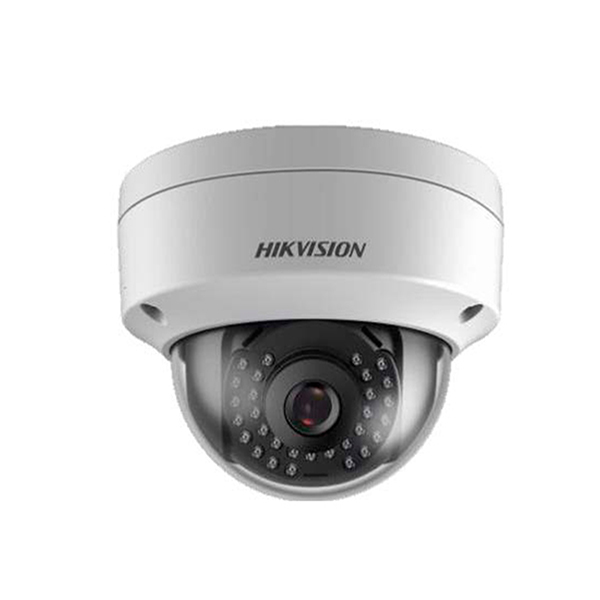
\includegraphics[width=4cm]{Componentes/20_camaraip_2mp.jpg} \\
\end{tabular}
\end{table}

\begin{table}[H]
\centering
\renewcommand{\arraystretch}{1.3}
\begin{tabular}{p{9cm} p{4.5cm}}
\textbf{NVR 16 Canales PoE+} \newline
\textit{Marca: Dahua / Hikvision} \newline
Grabador de video en red con HDD 4TB, ubicado en el gabinete MDF para gestión centralizada. &
\centering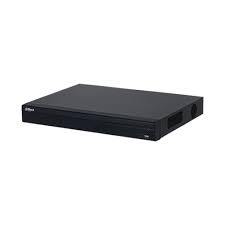
\includegraphics[width=4cm]{Componentes/21_nvr_16canales.jpg} \\
\end{tabular}
\end{table}

\subsubsection*{Canalizaciones}

\begin{table}[H]
\centering
\renewcommand{\arraystretch}{1.3}
\begin{tabular}{p{9cm} p{4.5cm}}
\textbf{Escalerilla Tipo Malla Electrozincada} \newline
\textit{Ancho: 300mm --- Norma: NEMA VE 1} \newline
Canalización principal (troncal) en pasillos, acero al carbono electrozincado. &
\centering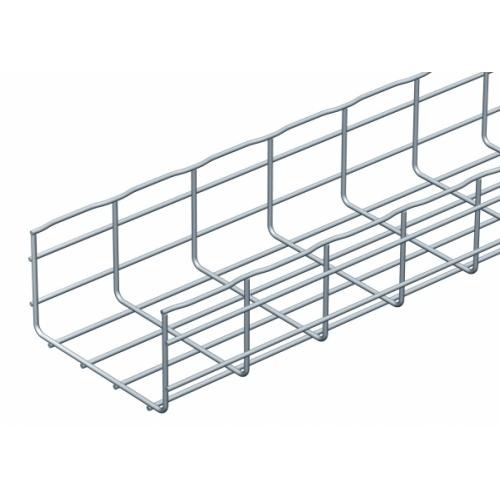
\includegraphics[width=4cm]{Componentes/22_escalerillaelectrozincada_300mm.jpg} \\
\end{tabular}
\end{table}

\begin{table}[H]
\centering
\renewcommand{\arraystretch}{1.3}
\begin{tabular}{p{9cm} p{4.5cm}}
\textbf{Canaleta PVC Doble Vía 40x20mm} \newline
\textit{Material: PVC rígido autoextinguible LSZH} \newline
Canalización secundaria con divisor físico para segregación datos/energía, adosada a pared. &
\centering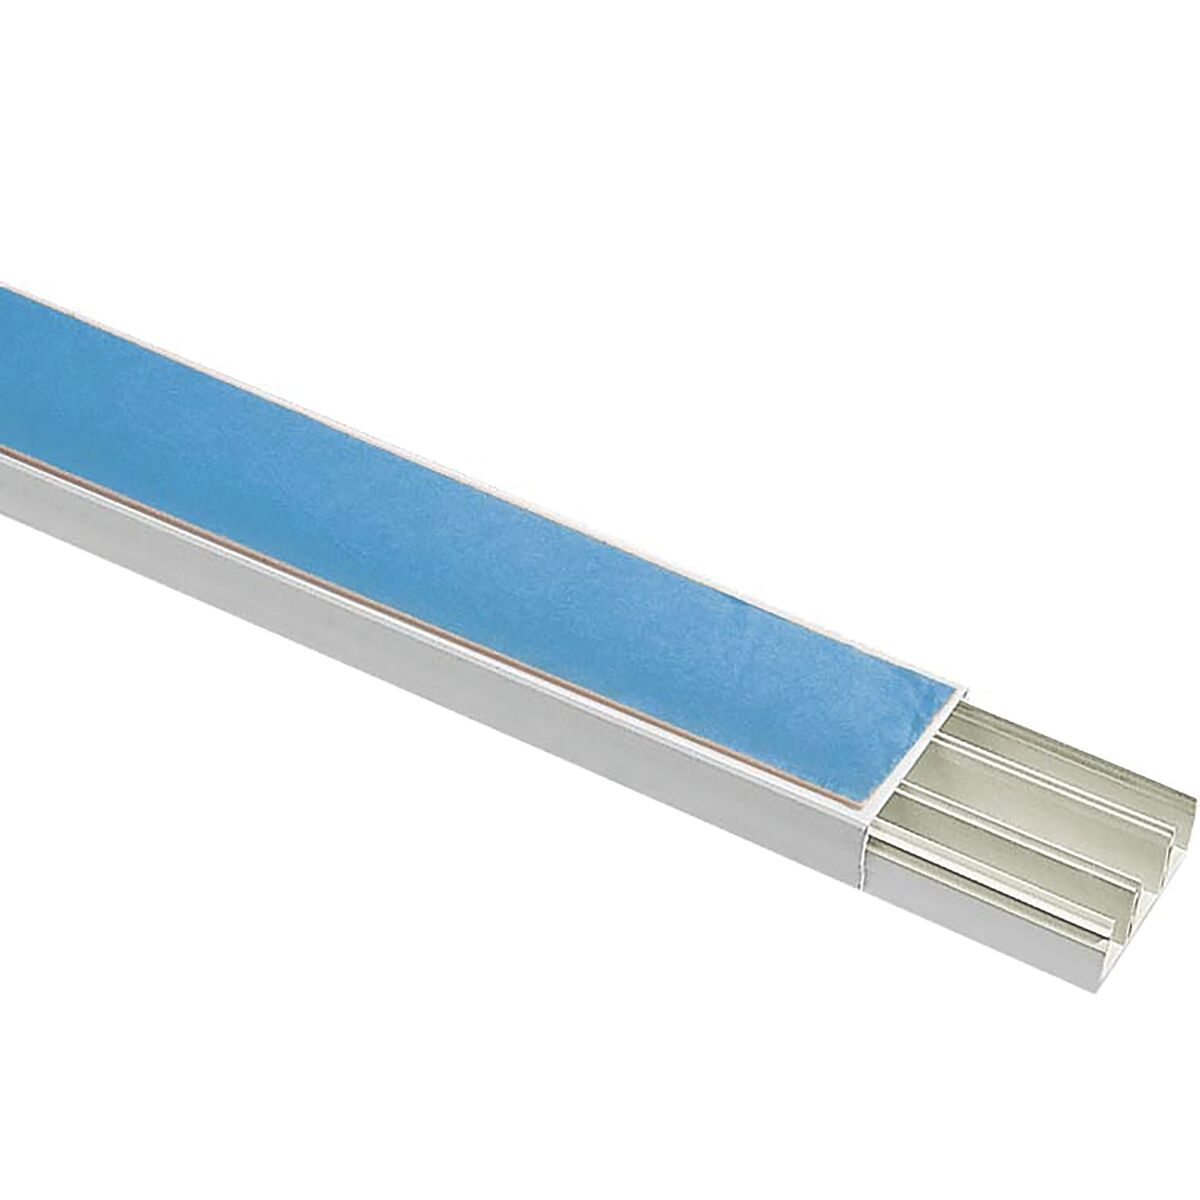
\includegraphics[width=4cm]{Componentes/23_canaletapvc_doblevia40x20mm_divisor.jpg} \\
\end{tabular}
\end{table}

\begin{table}[H]
\centering
\renewcommand{\arraystretch}{1.3}
\begin{tabular}{p{9cm} p{4.5cm}}
\textbf{Tubería Conduit EMT 1''} \newline
\textit{Material: Metálica} \newline
Protección del backbone de fibra óptica en pases verticales entre pisos. &
\centering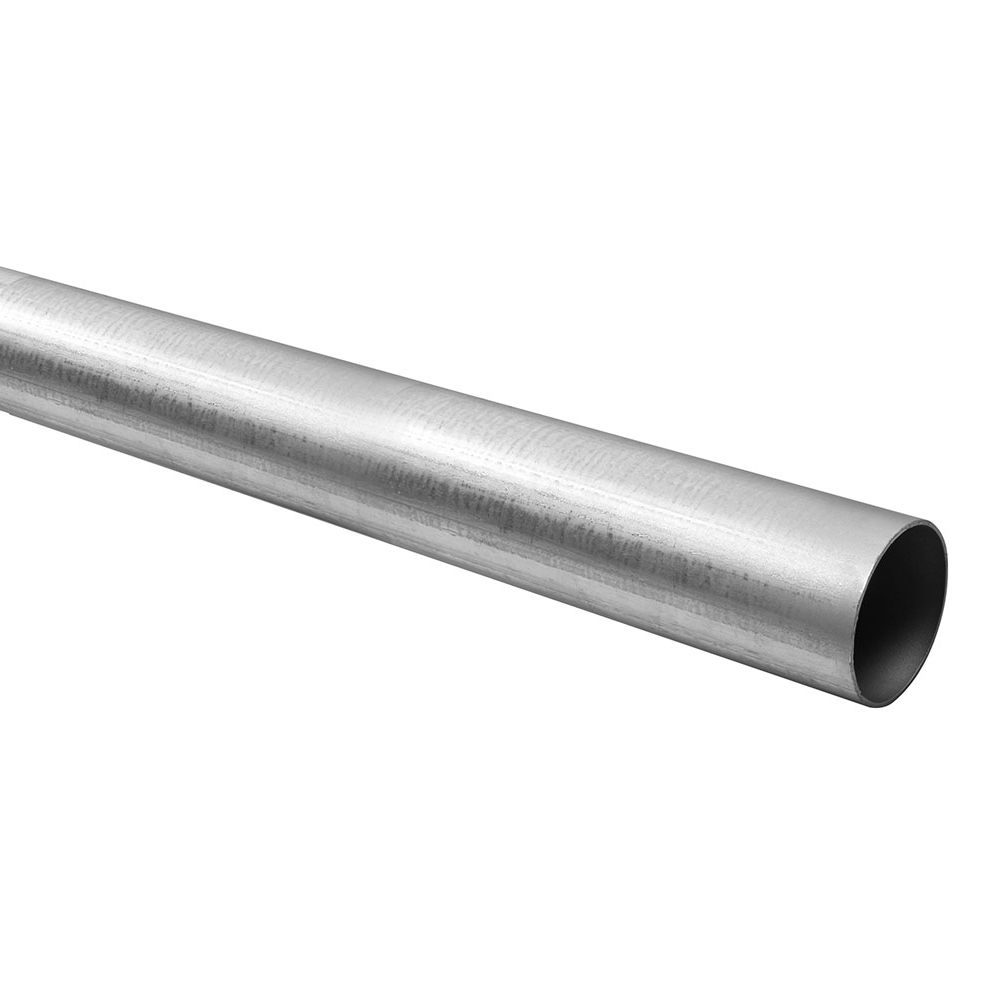
\includegraphics[width=4cm]{Componentes/24_tuberiaconduit_emt1''.jpg} \\
\end{tabular}
\end{table}

\begin{table}[H]
\centering
\renewcommand{\arraystretch}{1.3}
\begin{tabular}{p{9cm} p{4.5cm}}
\textbf{Caja de Registro Metálica} \newline
\textit{Uso: Paso y derivación de cableado} \newline
Instalada cada 15 m lineales de canalización y en cambios de dirección superiores a 30°. &
\centering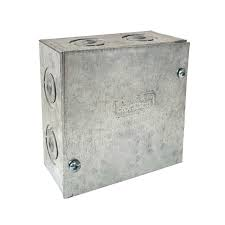
\includegraphics[width=4cm]{Componentes/25_cajaregistro_metalica.jpg} \\
\end{tabular}
\end{table}

\begin{table}[H]
\centering
\renewcommand{\arraystretch}{1.3}
\begin{tabular}{p{9cm} p{4.5cm}}
\textbf{Sello Cortafuego Intumescente} \newline
\textit{Uso: Pases de losa entre pisos} \newline
Mantiene la clasificación de resistencia al fuego de la estructura (mínimo RF-120). &
\centering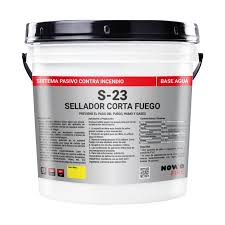
\includegraphics[width=4cm]{Componentes/26_selloconrtafuego_intumescente.jpg} \\
\end{tabular}
\end{table}

\subsubsection*{Certificación}

\begin{table}[H]
\centering
\renewcommand{\arraystretch}{1.3}
\begin{tabular}{p{9cm} p{4.5cm}}
\textbf{Certificador de Cableado Nivel IV} \newline
\textit{Marca: Fluke Networks --- Modelo: DSX-8000} \newline
Equipo de certificación de campo para validación de enlaces Cat 6A hasta 500 MHz. &
\centering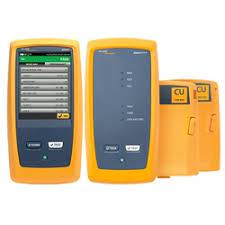
\includegraphics[width=4cm]{Componentes/27_certificadorfluke_dsx-8000.jpg} \\
\end{tabular}
\end{table}
